%!TEX root = ../dissertation.tex

\chapter{Implementation}
\label{implementation}

This chapter will start with a brief overview on how the whole system for this thesis is implemented and flows, detailing then further each of the procedures. It goes through the implementation of a simulator that is used to test the estimation algorithms in closed and controlled environment, the specifications of the real system setup and also the conception of a C++ library that deals with all of this.

As a reminder, the coordinate system convention that will be used throughout this chapter is the computer vision one mentioned in section \ref{cha2:represent}. 

\section{Flow Overview}
\begin{figure}[ht]
	\centering
	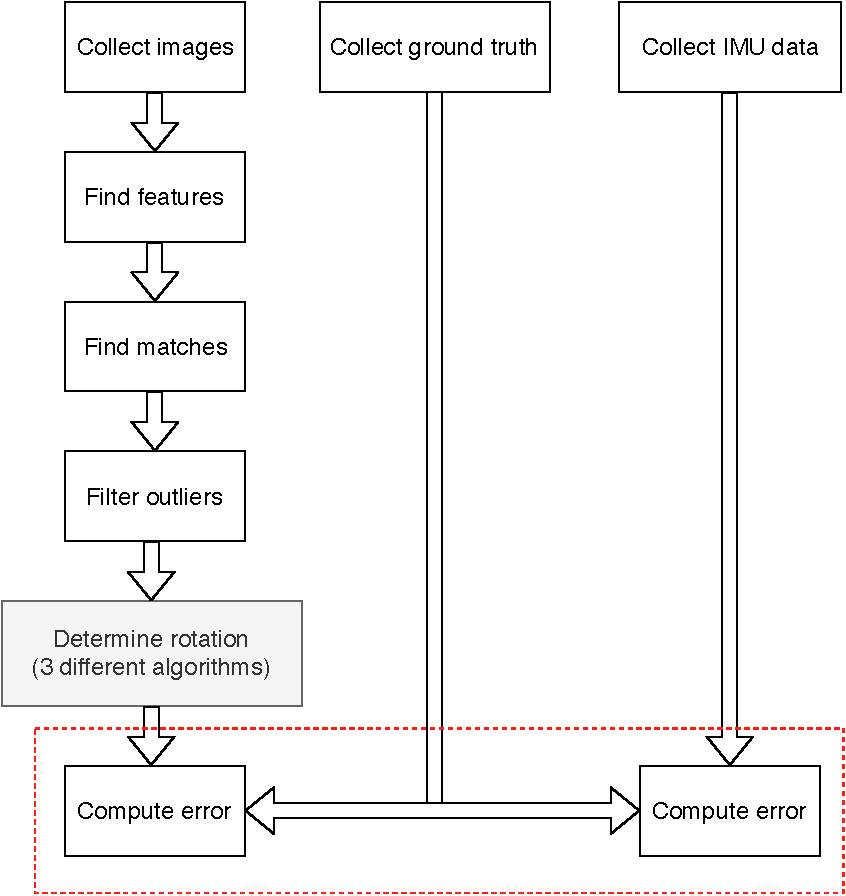
\includegraphics[width=0.7\textwidth]{images/approach.pdf}
	\caption[Flow Diagram]{Flow Diagram. The \acrshort{rgb} camera collects two images, before and after rotation. In each image, features are detected and matched between them. Some matches might be false or have too much noise, so they are filtered out. Using the matches information, the executed rotation is determined using an estimation algorithm. 3 algorithms will be tested. Finally, the estimated rotation is compared against the ground truth. The \acrshort{imu}'s orientation output is also compared against the ground truth to evaluate its performance in relation to the camera.}
	\label{cha3:methodology:approach}
\end{figure}
Figure \ref{cha3:methodology:approach} shows the flow of the procedures that determine the eye rotation. Firstly two images are collected, before and after rotating. In each of the images, points that make the image unique and identifiable, called feature points, are detected. These points are then matched together between the images. Because some may be wrongly matched, as mentioned on section \ref{cha2:robustest}, they need to go through a filtering process. Afterwards, the rotation can be determined using one of the algorithms presented on section \ref{methods}. In order, to select the best algorithm their errors are all compared against the ground truth. Besides that, the \acrshort{imu} data is collected to compare its performance against the camera.\\

This workflow specifies what is needed to determine the rotation of the camera for real data sets. However, in order to evaluate the three algorithms in a controlled environment, a simulator was implemented which generates image points matches with known rotations. These points may contain additive Gaussian noise, or even false matches to test the performance of the outlier filtering and the resilience of the estimator. 

Both the simulator and the procedures to deal with real data were implemented in Matlab \footnote{\href{https://www.mathworks.com/products/matlab.html}{https://www.mathworks.com/products/matlab.html}} and can be found in the thesis github repository\footnote{\href{https://github.com/Mrrvm/Orient/tree/master/Matlab}{https://github.com/Mrrvm/Orient/tree/master/Matlab}}. A C++ library was also created to deal with the data on the real system for convenience and computational speed, and can also be found at the repository\footnote{\href{https://github.com/Mrrvm/Orient/tree/master/C++}{https://github.com/Mrrvm/Orient/tree/master/C++}}.

\section{Simulator}
\label{rienreive}
\begin{minipage}{0.5\textwidth}
	\centering
	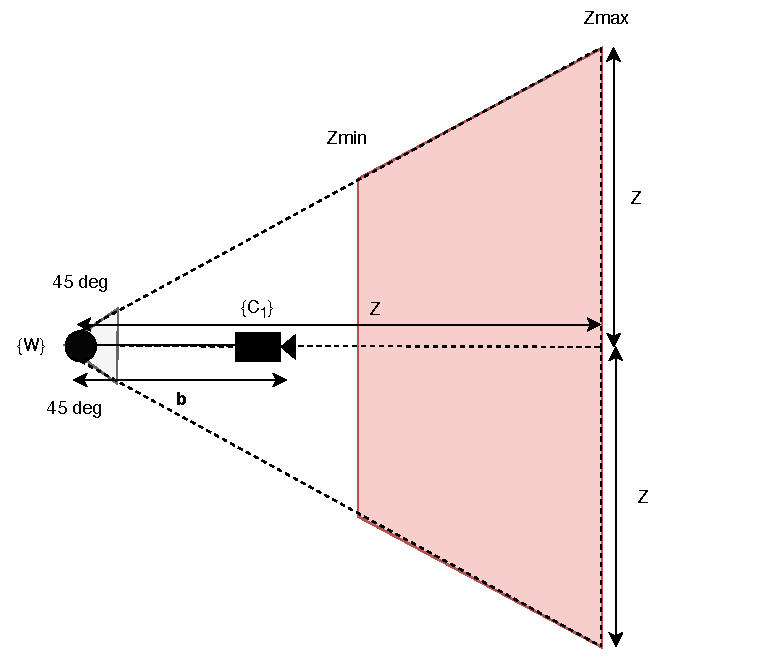
\includegraphics[width=0.9\textwidth]{images/rangesim.pdf}
	\captionof{figure}{Range in which simulated points are generated}
	\label{cha4:sec3:rangesim}
\end{minipage}
\begin{minipage}{0.5\textwidth}
	\centering
	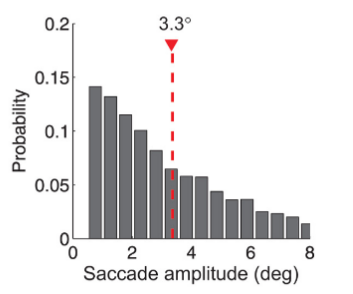
\includegraphics[width=0.6\textwidth]{images/freeview.png}
	\captionof{figure}{Probability of executing a specific \gls{saccade} amplitude under free viewing \cite{saccadeamp}}
	\label{cha4:sec3:freeview}
\end{minipage}\\

To generate corresponding points in two simulated images, first it's necessary to pick the rotation amplitude between them. This amplitude is drawn from a normal distribution with a certain variance, which simulates a naturalistic real environment. Poletti, M. et al \cite{saccadeamp}, provides information on the probability of specific \gls{saccade} amplitudes when free viewing. Free viewing is measured during normal examination of a scene, the observers freely view pictures of natural scenes, each presented for $10 \ s$. The mean of the distribution is $3.3 \ degrees$, shown on figure \ref{cha4:sec3:freeview}.

Afterwards, 3D points represented in the world reference frame, ${W}$, are generated within a camera viewing range of $90 \ degrees$, as represented on figure \ref{cha4:sec3:rangesim} in both $Y$ and $X$ directions, and within a range of depth $Zmin$ and $Zmax$, in order to represent a real environment where objects are at certain distances, that may affect the accuracy of the estimation. This suffices range to simulate real eye saccades, given the amplitudes are small as seen before. 

Having the points in the world frame, they are then represented in the camera reference frame before rotating, ${C_1}$, and after rotating, ${C_2}$, according to the amplitude designated between them. Finally, the 3D points are projected into the 2D image plane, and it's verified if they fit the image dimensions chosen for the simulated images.

It's possible to add Gaussian noise and also false matches into the simulator. For the former, random values taken from a Gaussian distribution, with a chosen variance for the simulation, are added randomly to one of the images, before or after rotating. In the case of false matches, they are set according to the quantity chosen for the simulation, and defined as a random 2D coordinate within the image dimensions that will replace an existing correct coordinate in a random match in one of the images.

The 2D point matches are now ready to be sent to the rotation estimator.

\section{Real system}

\subsection{Setup}
As shown on Figure \ref{cha1:sec1:fig:curr_eye_model}, the current eye prototype is composed by 3 motors that move the 6 elastics, coupled as 3 muscle pairs. To the center of rotation seen on Figure \ref{cha4:sec3:eyescheme} is attached a camera, and an \acrshort{imu}. The distance from the center of rotation to the camera, defined previously as baseline length, is $[0 \ 0 \ 53.7] \pm 3 \ mm $. The camera reference frame and the \acrshort{imu} reference frame differ. 
This setup was fixed $5 \ m$ away from furthest object in the scene.
\begin{figure}[ht]
	\centering
	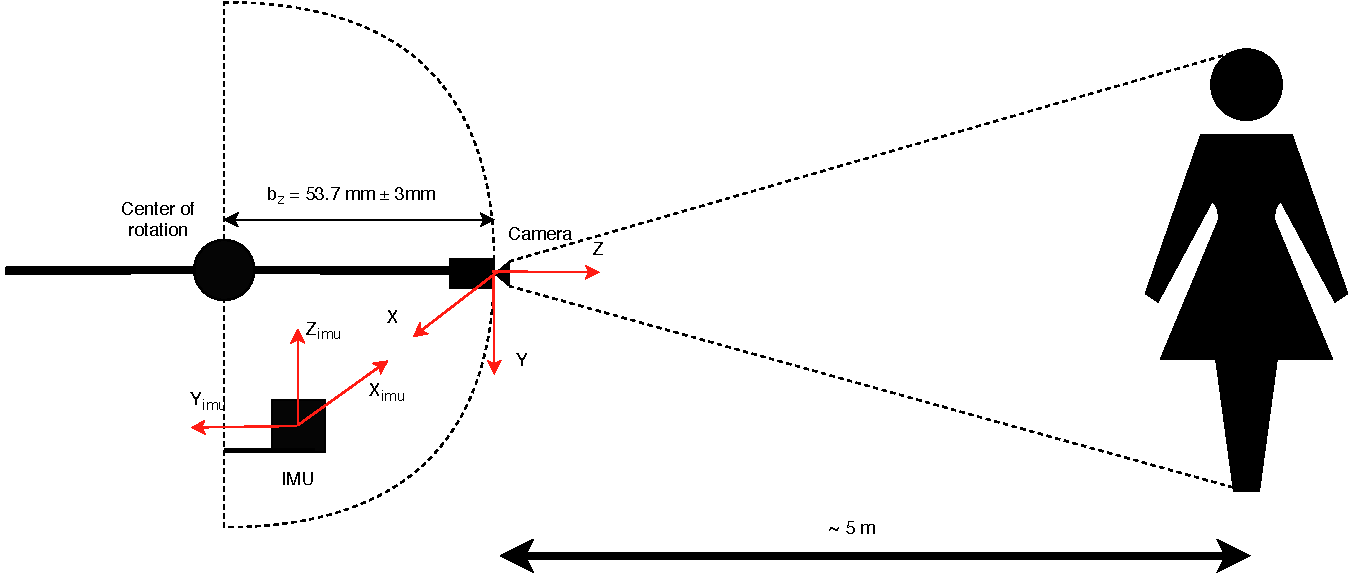
\includegraphics[width=\textwidth]{images/eyescheme.pdf}
	\caption[Eye prototype scheme used on the experiments]{Eye prototype scheme used on the experiments. The camera is displaced from the center of rotation by $b_z$ }
	\label{cha4:sec3:eyescheme}
\end{figure}

The camera was calibrated\footnote{See appendix \ref{appendix:cha2:calibration} for more details on this} and the images were collected using an uEye LE USB3 camera\footnote{See appendix \ref{appendix:cha2:camera} for camera specifications.} in grayscale before and after a certain rotation.

\subsection{Collect ground truth}
\label{rnfrfref}
Using the same camera in the same positions, two images were taken with a chessboard \footnote{See appendix \ref{appendix:cha2:chessboard} for chessboard specifications.} on the scenery, which is used to determine the ground truth through its regular pattern. The ground truth is then used to evaluate the estimation algorithms performance and also the \acrshort{imu}'s performance over the camera. On Figure \ref{cha3:methodology:imagesex}, an example of two collected image pairs can be observed. It's important to note that there is error associated to the ground truth that can heavily affect the outcome of the experiments.
	
\begin{figure}[ht]
	\centering
	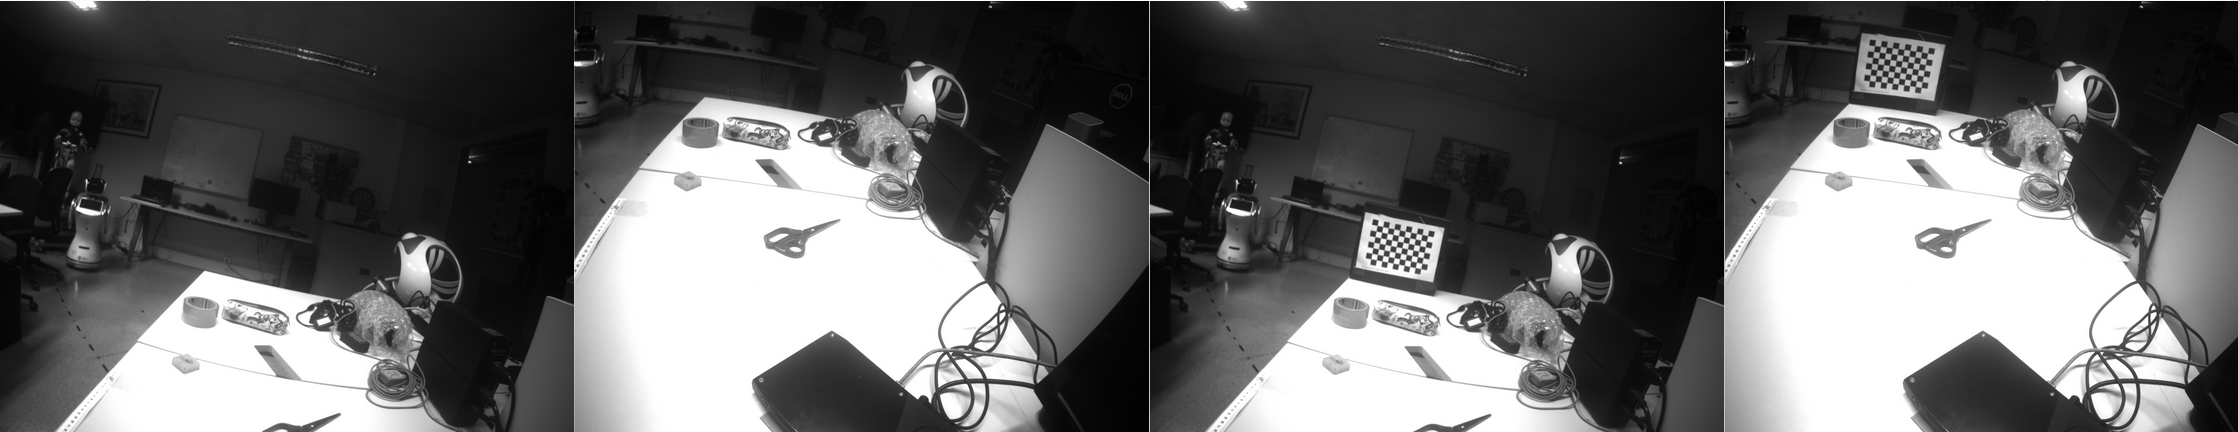
\includegraphics[width=\textwidth]{images/imagesex.png}
	\caption[Example of of two collected image]{Example of two collected image. The first and second images are used to find feature matches and estimating the orientation. The third and fourth images are the same as the first and second ones, respectively, but with a chessboard on the scene, that can serve as ground truth to evaluate the algorithms and the \acrshort{imu}'s performance.}
	\label{cha3:methodology:imagesex}
\end{figure}

To determine the ground truth from the images with the chessboard using Matlab, the following steps were taken.

\begin{enumerate}
	\item Checkboard points are detected using \texttt{detectCheckerboardPoints}\footnote{\href{https://www.mathworks.com/help/vision/ref/detectcheckerboardpoints.html}{https://www.mathworks.com/help/vision/ref/detectcheckerboardpoints.html}} by Geiger A. et al \cite{geiger} for each image;
	\item The extrinsic parameters are determined using \texttt{extrinsics}\footnote{\href{https://www.mathworks.com/help/vision/ref/extrinsics.html}{https://www.mathworks.com/help/vision/ref/extrinsics.html}} for each of the images. This function outputs a rotation matrix that allows the transformation from the world coordinate to the camera coordinate frame before rotating, $^{C_1}_{W}R$ and after rotating, $^{C_2}_{W}R$;
	\item The rotation from the camera's position before rotating to its position after rotating is computed as
	\begin{equation}
		^{C_1}_{C_2}R = (^{W}_{C_1}R)^T  \cdot  ^{W}_{C_2}R
	\end{equation}
	and used as ground truth to compare with the rotations determined by the estimation algorithms.
\end{enumerate}

\subsection{Feature detection, matching and filtering}
\label{cha3:features}

It is necessary to gather corresponding features in consecutive images taken before and after a rotation, and to use an algorithm to estimate the orientation using those features. The latter, also referred to as keypoints or interest points, are spatial locations of an image that ``stand out", allowing them to be identifiable. These points should be such that even after rotating, translating, shrinking or distorting the image, they can be found.

It is crucial absolutely needed to have a solid detection and trust-worthy correspondence of image features (matching) when making an ``eye" movement to eventually estimate the its current orientation. Two main approaches exist to the problem of feature detection and matching. The first method finds features in one image and matches these features in the other image. The second method, which is more suitable for points in the near space, independently detects features in both images and subsequently matches them on the basis of local correspondences.

It might not be appropriate to extract features from an image having high detail (i.e. high spatial bandwidth) on the finest stable scale possible, because when matching features with another image at a different (coarser) scale those details may no longer be detectable. Therefore, it's important to extract features at a variety of scales to ensure their invariance. 

Besides scale, preserving rotation and orientation invariance is also a concern. One way to deal with this problem is to define a descriptor. This is a scaled and oriented patch around the chosen point with the local orientation and scale, from which the dominant orientation can be extracted to guarantee its invariance. \cite{multiview}

There exist a multitude of algorithms that can do the job. However, none of these algorithms is optimal for all images, as each of them is optimized for particular computer vision applications, with performance depending heavily on the environmental properties (illumination, image quality, contrast, ...). A comprehensive survey on the state of the art of feature detection and description  \cite{featsift} (by Salahat E. and Qasaimeh M. in 2017), proposes that ideal features should have the following properties:
\begin{itemize}
	\item Distinctiveness: the gradient variations surrounding the point should be sufficiently large;
	\item Locality: to avoid obstruction and deformation between the two images.
	\item Quantity: enough features to describe the content;
	\item Accuracy: features should be accurate enough to be detected independently of image scale, shape or pixel location;
	\item Efficiency: be detected fast enough for real-time systems;
	\item Repeatability: a high percentage of features should be detected in both images on the overlapping regions;
	\item Invariance: deformative effects on the features, due to scaling, rotation or translation are minimized;
	\item Robustness: features should be less sensitive to deformations due to noise, blur, compression, and so on.
\end{itemize} 
The review paper also presents an overview on the recent algorithms proposed on this matter, comparing them in terms of the metrics defined above. The analysis in that article suggests that Maximally stable extremal regions (MSER) and \acrfull{sift} algorithms enhance performance on computational complexity, accuracy and execution time. From the scale and rotation invariant algorithms, \acrfull{surf}, proved to be faster than \acrshort{sift}, although not as robust.

MSER, by Matas J. et al in 2002 \cite{mser}, are areas of uniform intensity outlined by contrasting backgrounds. They are constructed by trying multiple thresholds on the input image. The ones that remain unchanged in shape over the range of thresholds are the potential features to be selected as areas of interest. The centroids of these areas can subsequently be used to create a feature descriptor for the matching step.

\acrshort{sift} (by Lowe, David G. et al in 2004) \cite{sift} algorithm detects image features using a Gaussian filter by generating increasingly blurred images, and subtracting each image to each other. This is done in several scales in order to provide scale invariance. Afterwards, a descriptor for each feature at a certain scale is created and includes information about the orientation and gradient magnitude around the point, which also grants rotation invariance.

\acrshort{surf} (by Bay, Herbert et al in 1999) \cite{surf} uses an integral image, which is an intermediate representation of the original image where the value of a location is the sum of all pixels of a rectangular region formed around that location. This is called box filter and serves as an approximation to the \gls{gauss}, speeding up the process in relation to \acrshort{sift}.

A more comprehensive explanation on both SIFT and SURF can be found at appendix \ref{appendix:cha1:sift} and \ref{appendix:cha1:surf}, respectively. Because \acrshort{surf} is faster and more accessible due to patenting concerns regarding \acrshort{sift}, it will be be used on this work.

\subsection{Matching step}
Regarding the matching of feature descriptors, one of the most common search algorithms used, that will also be used here, is the Nearest Neighbor Search. \acrfull{flann} \cite{flann} provides a library for performing this kind of searches in high-dimensional spaces. It contains a collection of algorithms that the authors found to  work best for nearest neighbor search and a system for automatically choosing the best algorithm and optimum parameters depending on the dataset.

\subsection{Collect IMU data}
The \acrlong{imu} \footnote{See appendix \ref{appendix:cha2:imu} for \acrshort{imu} specifications.} obtains two quaternions (see section \ref{cha2:represent:quat}) with the current camera's orientation before and after rotating, coherently with the images. To estimate the rotation between the two positions of the camera, the rotation quaternion is simply computed by \ref{inrefiorenf}. 

The \acrshort{lpmscu} \acrshort{imu} offers a C++ library, the LpSensor library, that contains classes that allow the integration of these devices into their own applications, and also wrappers for other platforms, yet the Matlab one is still under development. Hence, the \acrshort{imu} data is obtained through C++ as it will be seen further ahead on section \ref{diwefneoinfof}.

\section{Filtering matches}
\label{rnfireonce}
As referred on section \ref{cha2:robustest}, robust estimation is essential to guarantee an accurate estimation by eliminating outliers that can interfere with the estimation. On that note, \acrshort{ransac} with \acrshort{oppr} is used to filter the matches.

Regarding the summary on section \ref{cha2:robustest}, \acrshort{ransac} was implemented the following way.

\begin{itemize}
	\item 3 matches are selected for the small random sample, as only three are necessary to estimate the rotation through \acrshort{oppr}.
	\item For the matches to be inliers, the projection of the points from the camera's first position to the second through the defined model must not differ more than $5 cm$.
	\item The quantity of matches necessary for the the model to be considered good and the quantity of iterations needed to, in principle, estimate it are designated as following.
	
	If the whole set of matches contains a fraction $\varepsilon$ of outliers, the probability, $P$, of at least one of the subsets of ``inliers" being tested generating a good model is 
	\begin{equation}
	P=1-\left[1-(1-\varepsilon)^{p}\right]^{iters},\\
	\end{equation}
	where $p$ is the quantity of needed matches for the model to be good and $iters$ is the number of iterations. \cite{detep}
	Making the probability near 1, the quantity of subsets - iterations - to test is
	\begin{equation}
	iters = \frac{\log (1-P)}{\log \left[1-(1-\varepsilon)^{p}\right]}.
	\end{equation}
	
	$P$ was considered $40\%$ and $p = 15$, which is half of the quantity of the maximum number of matches allowed, due to speed concerns. 
\end{itemize}

\section{Determine the rotation}
To estimate the rotation, the three different methods \acrshort{oppr}, \acrshort{mbpe} and \acrshort{grat} were used. For the last two, it is necessary to initialize them with \acrshort{oppr} as mentioned on section \ref{MBaPE}, and for \acrshort{oppr} and \acrshort{mbpe} it is necessary to project the points onto a sphere with a large enough radius. \acrshort{oppr} is easily implemented using \acrshort{svdd}. However, the others are non-linear unconstrained minimization problems, thus a non-linear solver is necessary. 

For that, Matlab's \texttt{fminsearch}\footnote{\href{https://www.mathworks.com/help/matlab/ref/fminsearch.html}{https://www.mathworks.com/help/matlab/ref/fminsearch.html}} was utilized. This function is an adaptation of the Nelder-Mead simplex algorithm, described by Lagarias et al. \cite{lagarias} \texttt{fminunc}, another possible function to use, implements the Newton method and deals with explicit boundaries. It usually is more suitable for problems with a large number of parameters and it needs to know the gradient of the cost function. However, \texttt{fminsearch} was chosen as it is simpler, gives less trouble to implement and should be enough for the current problem.

\acrshort{oppr} outputs a rotation matrix from the \acrshort{svdd}.
\acrshort{grat} requires the computation of the fundamental matrix, thus it is necessary to have a rotation matrix previously, as expressed on \ref{dopewnrvno}. For \acrshort{mbpe}, it's also easier to use a rotation matrix to calculate the points back projections. Hence, this rotation representation is the most suited for the problem. Yet, in order to estimate only 3 parameters instead of 9, the Euler angles representation (see section \ref{cha2:represent}) in the ZYX convention is used as the variable to estimate. This has several advantages, while debugging it's easier to understand how the results of the estimations differ from each other and the ground truth, and during the optimizations by converting the Euler angles into a rotation matrix, it guarantees the constraint that the matrix being determined is in fact, a rotation matrix, satisfying the conditions \ref{epwifneprnf} and \ref{ienvpirnf}.

\section{Compute the error}
The error is then calculated as
\begin{equation}
	error = ||{\mathbf{ \theta}_{gt}-\mathbf{ \theta}_{est}}||,
	\label{firenr}
\end{equation}
where $\mathbf{ \theta}_{gt}$ are the ground truth Euler angles and $\mathbf{ \theta}_{est}$ are the Euler angles of the estimation.


\section{C++ Library}
\label{diwefneoinfof}

So that in the future, it becomes more convenient to estimate the orientation of the camera on the actual prototype, which is an essential aspect of this work, a C++ library was implemented. It provides a number of classes that wrap and simplify the code, along with documentation and basic usage examples. The idea was to create it open-source, in such a way that it may help whomever uses the same hardware, or wants to do similar estimations.

It is organized into 4 different classes, \texttt{Camera}, \texttt{Sensor}, \texttt{Image} and \texttt{Rotation}, that provide all the data in the same computer vision friendly format. In other words, it makes everything compatible with the very popular \acrlong{opencv}\footnote{\href{https://opencv.org/}{https://opencv.org/}}, that contains up to 2500 optimized algorithms for this type of work.


\begin{itemize}
	\item Class \texttt{Camera} deals with all the little details of using uEye camera software, reducing it to a couple of easy-to-use functions: \texttt{Connect()} and \texttt{Disconnect()}, \texttt{Capture()} for capturing images, \texttt{SpawnCameraError()} for debugging camera errors and finally \texttt{Calibrate()}, for calibrating the camera given a bunch of chessboard images\footnote{See appendix \ref{appendix:cha2:calibration}}.
	
	\item Class \texttt{Sensor} again wraps all the work fo dealing with the LpSensor Library, into 3 functions, \texttt{Connect()}, \texttt{Disconnect()} and \texttt{GetOrientation()}.
	
	\item Class \texttt{Image} holds an image object with which it's possible to execute several functions within the range of this work, such as \texttt{FindKeypoints()}, \texttt{FindMatches()}, \texttt{ShowMatches()} and \\
	\texttt{DetectChessboardRotation()} for obtaining the ground truth as mentioned on section \ref{rnfrfref}. It essentially processes the data comming from the \texttt{Camera} class.
	
	\item Class \texttt{Rotation} implements the three estimation algorithms and some auxiliary functions:\\ \texttt{RansacByProcrustes()},  \texttt{ProjectToPlane()}, \texttt{ProjectToSphere()}, \texttt{MakeHomogeneous()} and \texttt{Estimate()} that estimates the rotation according to the algorithm chosen.\\
	To implement the \acrshort{mbpe} and \acrshort{grat} into C++, it was again necessary to use a non-linear optimizer. For that it was made use of Ceres Solver\footnote{\href{http://ceres-solver.org/}{http://ceres-solver.org/}}, which is a very complete and well-documented library produced by Google since 2010, that can solve non-linear least squares.
	
\end{itemize}




















